% *****************************************************************************
%     sections/chapter2.tex
%
% Last edit: 16/03
% *****************************************************************************

\chapter{Bayesian inference of neutron star observables} % 1

\section{From the equation of state to neutron star observables} % 0.75

% EoS microscopic -> one wants to evaluate macroscopic properties of the star,
%   such as its mass or radius.
% hydrostatic equilibrium
% plan

\subsection{Masses and radii} % 4

% introduction: mass is the observable that is the most accessible for
% astronomers.
% -> mass with the Shapiro delay technique
% -> radius with Nicer, tidal, etc.

% we can calculate masses and radii from the EoS (the only necessary input) by 
% integration of the tov equation throughout the star (explain TOV equation)
The NS masses and radii are given by the solution of the hydrostatic
equilibrium equations in general relativity (GR) for spherical and nonrotating 
stars~\cite{Tolman1939,Oppenheimer1939},
%
\begin{eqnarray}
  \frac{dP}{dr} &=& -\frac{G\rho_B m}{r^2}\left(1 + \frac{P}{\rho_B
  c^2}\right)\left(1+\frac{4\pi
  Pr^3}{mc^2}\right)\left(1-\frac{2Gm}{rc^2}\right)^{-1},\label{eq:tov}\\
      \frac{dm}{dr} &=& 4\pi r^2\rho_B,\label{eq:massbal}\\
  \frac{d\Phi}{dr} &=& -\frac{1}{\rho_B
    c^2}\frac{dP}{dr}\left(1+\frac{P}{\rho_B
  c^2}\right)^{-1}\label{eq:metric},
\end{eqnarray}
%
where $G$ is the gravitational constant, $P$ the pressure, $\rho_B c^2$ the
energy density, and $m(r)$ the is the gravitational mass inside the sphere of
radius $r$, defined within the Schwarzschild metric $ds^2 = c^2dt^2e^{2\Phi} 
- e^{2\lambda}dr^2 - r^2(d\theta^2 + \sin^2\theta d\phi^2)$. The function 
$\Phi(r)$ corresponds to the gravitational potential, and $\lambda(r)$ is 
related to the enclosed mass $m(r)$ through
%
\begin{equation}
  e^{-\lambda} = \sqrt{1-\frac{2Gm}{rc^2}}.
\end{equation}
%
% description of the equations
Eq.~(\ref{eq:tov}) is the so called Tolman-Oppenheimer-Volkoff (TOV) equation 
of hydrostatic equilibrium. The integration of Eq.~(\ref{eq:massbal}) from
$r=0$ to the boundary $r=R$, $R$ being the NS radius, gives the total mass
$M=m(R)$ of 
the star. Eq.~(\ref{eq:metric}) is a relativistic equation for the metric function 
$\Phi(r)$. Here, we focus on solving Eqs.~(\ref{eq:tov}) and 
(\ref{eq:massbal}), which gives the profiles $P(r)$, $\rho_B(r)$, and $m(r)$ 
for a given EoS, $P(\rho_B)$, the determination of which was discussed in detail 
in Chapter 1.

% explain numerical method for a central density nc (CGS, Euler method, lagrangian interpolation)
In view of solving the hydrostratic equilibrium equations for a given tabulated 
EoS, one first have to choose an arbitrary value for the central density $\rho_{B,c}$ and 
interpolate the central pressure $P_c = P(\rho_{B,c})$, corresponding to $r=0$, 
with the associated boundary condition $m(r=0) = 0$. Then, using a Runge-Kutta 
method, one integrate up to $r=R$, defined as $P(r=R) = 0$ (our numerical 
condition is $P < 5\times 10^{-4}$ MeV/fm$^{3}$, which is a sufficiently low 
value of the pressure). At each new step of pressure, one has to interpolate 
the mass density $\rho_B$ in the table. In the end, for a given value of central 
density $\rho_{B,c}$, one obtains the profiles $P(r)$, $\rho_B(r)$, and $m(r)$, 
and therefore a value for the NS mass $M$ and radius $R$. The typical values 
of these observables are $M=1.4M_\odot$ and $R=10$ km~\cite{Haensel2007}.\\
% The problem is that the central density inside a NS is not known... thats why 
%   we are interested in the Mass radius relation
In fact, the central density inside a specific NS is not known, and is expected
to range from $\approx 4.6\times 10^{14}$ g/cm$^3$ to $\approx 4\times 10^{15}$
g/cm$^3$. For this reason, we are rather interested in the mass-radius relation, which
can be obtained by calculating $M$ and $R$, following the numerical method
previously explained, for this range of central mass densities.\\
% efld
Let us recall that one has to redefine the high-order parameters $Q_{sat(sym)}$ 
and $Z_{sat(sym)}$ in order to reproduce existing functionals at densities
greater than $2n_{sat}$ with the metamodeling technique. This corresponds to
the ELFd technique introduced in \cite{Margueron2018a}.

\begin{figure}[!t]
\begin{center}
  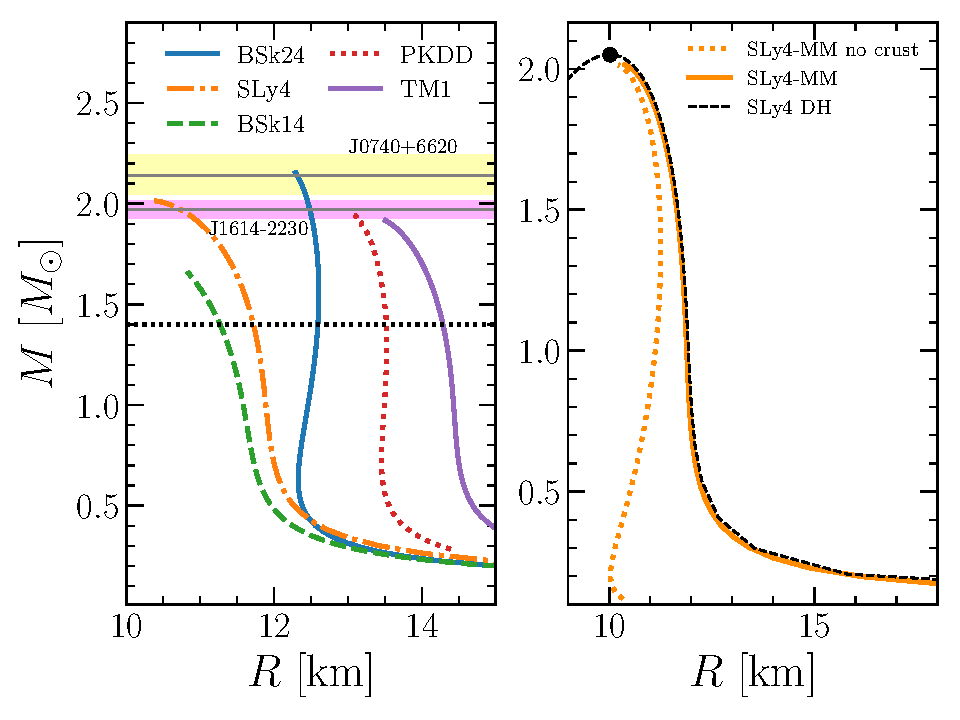
\includegraphics[width=0.9\linewidth]{figures/mr_popular.pdf}
\end{center}
\caption[Mass-radius relation for several popular EoS]{Left: Mass-radius 
  relation for several popular EoS calculated
  with the metamodeling technique. The black dotted line corresponds to the NS 
canonical mass, that is $1.4M_\odot$. The magenta band represents the measured 
mass of J1614-2230, $(1.97 \pm 0.04)M_\odot$ \cite{Demorest2010}, and the 
yellow band that of J0740+6620, $2.14_{-0.09}^{+0.10}M_\odot$ ($68.3\%$ 
credibility interval) \cite{Cromartie2020}.
Right: Mass-radius relation for the DH EoS for SLy4 functional (black dashed
line), and the SLy4 EoS calculated with the metamodeling technique (solid
orange line). The black circle indicates the maximum mass.}\label{fig:mr_popular}
\end{figure}
 
The left panel of Fig.~\ref{fig:mr_popular} shows the mass-radius relation for 
several popular EoS based on Skyrme-type functionals BSk24, SLy4, and BSk14, 
and relativistic models PKDD and TM1, calculated within the metamodeling 
technique. A strong model dependence is observed, with radii of canonical NS 
ranging from $R_{1.4}=11.5$ km for BSk14 to $R_{1.4}=14.5$ km for TM1. More
specifically, it is seen that the radius is positively correlated to the slope 
of the symmetry energy $L_{sym}$.\\
The bands correspond to the measured masses of the two most massive
pulsars observed to the present day. The mass of J1614-2230 was precisely 
estimated to $(1.97\pm 0.04)M_\odot$~\cite{Demorest2010}, and the very recent
relativistic Shapiro delay measurements of J0740+6620 led to 
$2.14_{-0.09}^{0.10}M_\odot$ ($68.3\%$ credibility
interval)~\cite{Cromartie2020}. Naturally, if an
EoS cannot insure such high masses, it should not be considered as reliable, 
in particular at high density, since the maximum mass is determined by the 
stellar core EoS. In particular, it is seen that the maximum mass corresponding
to the BSk14 functional, $1.8M_\odot$, is lower than the measured mass
of J1614-2230. Also, while the SLy4 EoS satisty this constraint, the maximum 
mass for this EoS, $2.05M_\odot$, is lower than that of J0740+6620. This 
outline the fact that measuring the mass of pulsars is important, because it 
provides a strong constraint on the stellar matter EoS. Similarly, the NICER
telescope is expected to provide, for years to come, a constraint on the NS
radii with a precision of $5\%$.

The mass-radius relation for the SLy4 EoS is represented in the right panel of
Fig.~\ref{fig:mr_popular}. The solid orange line corresponds to $M(R)$ for the 
SLy4 EoS calculated within the metamodeling technique, and the dashed 
black line is the calculation based on the DH EoS for SLy4 functional. A perfect
agreement is observed between the two curves, reflecting the small error on the
EoS, illustrated in Fig.~\ref{fig:unified}. \\
The dotted orange line shows the mass-radius relation for the SLy4 EoS without
considering the clustering of matter at low density, that is assuming that the
NS star interior consists of $npe\mu$ matter at all densities. In that case,
for a canonical NS, we find $R_{1.4} = 11.1$ km, which is almost $1$ km lower 
with respect to the result with a crust EoS. Moreover, this difference is found 
to be larger with decreasing mass. This shows that the crust EoS is essential 
to properly predict NS radii. However, we can see that the NS maximum mass is 
entirely determined by the stellar core EoS.\\
The black point marks the maximum mass for the SLy4 EoS, $M_{max} = 2.05M_\odot$. 
Let us notice that the branch left to the point is unstable, 
because from this point the mass decreases with central density increasing.

% As mentionned in Chapter 1, a pricese estimation of the crust-core transition 
% point is essential if one is interested in crustal properties. Explain how
% crust thickness + FIGURE
As explained in Chapter 1, a precise estimation of the CC transition point is
required as far as crustal properties are concerned. In particular, the crust
thickness blabla.

% Finally, a word about alternative theories of gravity (rainbow, f(R), etc.)

\subsection{Moment of inertia} % 2

% explain why are we interested in the determination of this observable
% maybe compare approximations to the complete integration of the equation
% results
% crust moment of inertia ('we will see in 2.3.3 that it is linked to blabla')
% results

\subsection{Tidal deformability} % 2

% observable of interest since gw170817 event
% explain tidal deformability (dimless, lambda1-lambda2, lambda tilde...)
% derive equations from k2 love number
% a word about I-love-Q relations?

\section{Bayesian modeling of the equation of state} % 0.75

\subsection{Principle of Bayesian inference} % 1.5

% expressions
% discussions

\subsection{Prior distribution from nuclear experiments} % 2

\subsection{Sensitivity analysis} % 3
% ... on the crust-core transition point?

\subsection{Filters} % 0.25

\subsubsection{Low-density filters from ab initio calculations} % 2.5

% discuss ab initio calculations (saturation properties, max is 0.2, etc.)
% should we consider the pressure as a filter or not? (bsk24 does not fit in
%   the band)
% +/- 10% to account for other ab initio calculations

\subsubsection{High-density filters from astrophysical observations and 
physical requirements} % 1.5

% symmetry energy positive is a debatable hypothesis (see remark of referee)
% maximum mass as a sharp filter? 1.97? 2.23?
% more constraints in the future with nicer and lvc

\subsection{Posterior distribution of empirical parameters} % 3

% discuss the importance of filters?

\section{General predictions for neutron star observables} % 0.75

% should i add a subsection 'Posterior distribution of NS observables'?

\subsection{Confrontation with GW170817 event} % 1

\subsubsection{Equation of state} % 1

\subsubsection{Mass-radius relation} % 1.5

% speed of sound expansion allows for phase transition, unlike the mm
% -> lower radius found in 1908.10352 could be the sign of a pt to quarks?

\subsubsection{Tidal deformability} % 2

% was measured for the first time for gw170817 event allowing to calculate the
%   m1-m2, lambda1-lambda2 relations

\subsection{Bayesian analysis of the crust-core transition} % 4

% surface figures (prior/posterior)
% corr(Pt,Ksym) (link with chapter 1)
% correlation with isovector bulk parameters is softened if one consider p as a
%   free parameters (see corr matrix)

\subsection{Crustal moment of inertia and pulsar glitches} % 4

% explain pulsar glitches phenomena
% give the hypothesis explaining the phenomena
% superfluid neutrons in the crust
% is the crust enough? -> bayesian approach to consider every models (not only
%   relativistic or skyrme functionals as two separate families)
% the crust moment of inertia is calculated following eq given in 2.1.2. the
%   calculation is stopped at the crust-core interface
% report results

\section{Conclusion} % 1

% word on machine learning
